% ===========================================================================
% MODELO DE RELATORIO  ·  ENE0046 Laboratorio de Eletronica  ·  2026/2
%
% Como usar
%   1. Preencha o bloco IDENTIFICACAO logo abaixo.
%   2. Deixe comentados os autores que nao existirem. Um autor fica centralizado,
%      dois dividem a linha, tres ocupam tercos.
%   3. Substitua o texto de cada secao pelo seu. As orientacoes que estao la
%      dizem o que se espera em cada uma.
%   4. Compile com pdflatex duas vezes, ou com latexmk -pdf.
%
% Estrutura
%   Roteiro 1 nao tem bancada: use so a subsecao 4.1 e a 5.1, e compare o calculo
%   analitico com a simulacao de projeto.
%   Roteiros 2 a 7 usam a estrutura inteira.
%
% O arquivo estilo-relatorio.tex e a imagem logo-unb.png devem estar na mesma
% pasta deste arquivo.
% ===========================================================================
\documentclass[11pt,a4paper]{article}
% !TeX root = modelo-relatorio.tex
% Formatacao do relatorio. Compile o modelo-relatorio.tex, nao este arquivo.
\usepackage[T1]{fontenc}
\usepackage[utf8]{inputenc}
\usepackage[brazil]{babel}
\usepackage[a4paper,top=1.6cm,bottom=1.8cm,left=2.1cm,right=2.1cm]{geometry}
\usepackage[default]{lato}
\usepackage{amsmath,amssymb}
\usepackage{siunitx}
\usepackage{graphicx}
\usepackage{booktabs,array,longtable,colortbl}
\usepackage{enumitem}
\usepackage{tcolorbox}
\usepackage{xcolor}
\usepackage{tikz}
\usepackage{titlesec}
\usepackage{fancyhdr}
\usepackage{caption}
\usepackage{etoolbox}
\usepackage[colorlinks=true,linkcolor=azul,urlcolor=azul,citecolor=azul]{hyperref}
\tcbuselibrary{skins,breakable}

\definecolor{azul}{HTML}{0A4B8C}
\definecolor{azulclaro}{HTML}{E8F0F8}
\definecolor{verde}{HTML}{0B7A4B}
\definecolor{cinza}{HTML}{5B6672}
\definecolor{cinzaclaro}{HTML}{F4F6F8}
\definecolor{vinho}{HTML}{B04A4A}
\definecolor{vinhoclaro}{HTML}{FBF2F2}

\sisetup{output-decimal-marker={,}, per-mode=symbol}
\setlength{\parindent}{0pt}
\setlength{\parskip}{6pt plus 1pt}
\setlist{itemsep=3pt, topsep=4pt, parsep=0pt, leftmargin=1.3em}
\renewcommand{\arraystretch}{1.25}
\linespread{1.06}

% ---- secoes numeradas com marcador colorido -------------------------------
\titleformat{\section}[hang]
  {\Large\bfseries\color{azul}}
  {\raisebox{-1pt}{\tikz\node[fill=azul,text=white,rounded corners=2pt,
     inner sep=3pt,minimum width=20pt,align=center]{\bfseries\thesection};}}
  {10pt}{}
\titlespacing*{\section}{0pt}{16pt plus 3pt}{6pt}
\titleformat{\subsection}{\large\bfseries\color{cinza}}{\thesubsection}{8pt}{}
\titlespacing*{\subsection}{0pt}{11pt plus 2pt}{3pt}

% ---- legendas -------------------------------------------------------------
\captionsetup{font=small,labelfont={bf,color=azul},labelsep=period,skip=6pt}

% ---- identificacao --------------------------------------------------------
\newcommand{\autorA}{}\newcommand{\matA}{}
\newcommand{\autorB}{}\newcommand{\matB}{}
\newcommand{\autorC}{}\newcommand{\matC}{}
\newcommand{\autorum}[2]{\renewcommand{\autorA}{#1}\renewcommand{\matA}{#2}}
\newcommand{\autordois}[2]{\renewcommand{\autorB}{#1}\renewcommand{\matB}{#2}}
\newcommand{\autortres}[2]{\renewcommand{\autorC}{#1}\renewcommand{\matC}{#2}}

\newcommand{\disciplina}{ENE0046 · Laboratório de Eletrônica}
\newcommand{\semestre}{2026/2}
\newcommand{\turma}{}
\newcommand{\roteironum}{}
\newcommand{\roteirotema}{}
\newcommand{\aturma}[1]{\renewcommand{\turma}{#1}}
\newcommand{\roteiro}[2]{\renewcommand{\roteironum}{#1}\renewcommand{\roteirotema}{#2}}

\newcommand{\umautor}[2]{%
  \begin{minipage}[t]{\dimexpr\linewidth-4pt\relax}\centering
    \parbox[t][30pt][t]{\linewidth}{\centering
      {\fontsize{10.5}{12.5}\selectfont #1}}\\[-2pt]
    {\color{cinza}\fontsize{9}{11}\selectfont\texttt{#2}}
  \end{minipage}}

\newcounter{nautores}
\newcommand{\blocoautores}{%
  \setcounter{nautores}{0}%
  \ifdefempty{\autorA}{}{\stepcounter{nautores}}%
  \ifdefempty{\autorB}{}{\stepcounter{nautores}}%
  \ifdefempty{\autorC}{}{\stepcounter{nautores}}%
  \ifnum\value{nautores}=0
    \begin{center}\color{vinho}\bfseries
      Preencha ao menos um autor no preâmbulo do arquivo.
    \end{center}
  \else
    \begin{center}
    \ifcase\value{nautores}\or
      % --- um autor: ocupa o centro
      \begin{minipage}{0.5\textwidth}\umautor{\autorA}{\matA}\end{minipage}%
    \or
      % --- dois autores: metades
      \begin{minipage}{0.42\textwidth}\umautor{\autorA}{\matA}\end{minipage}\hspace{0.04\textwidth}%
      \begin{minipage}{0.42\textwidth}\umautor{\autorB}{\matB}\end{minipage}%
    \or
      % --- tres autores: tercos
      \begin{minipage}{0.31\textwidth}\umautor{\autorA}{\matA}\end{minipage}\hspace{0.015\textwidth}%
      \begin{minipage}{0.31\textwidth}\umautor{\autorB}{\matB}\end{minipage}\hspace{0.015\textwidth}%
      \begin{minipage}{0.31\textwidth}\umautor{\autorC}{\matC}\end{minipage}%
    \fi
    \end{center}
  \fi}

% ---- cabecalho do relatorio -----------------------------------------------
\newcommand{\capa}{%
\begin{tcolorbox}[colback=azul,colframe=azul,boxrule=0pt,arc=4pt,
  left=16pt,right=16pt,top=13pt,bottom=13pt]
\color{white}
\begin{minipage}{0.76\textwidth}
  {\fontsize{9}{11}\selectfont\textbf{\MakeUppercase{\disciplina{} · \semestre{}}}}\\[6pt]
  {\fontsize{22}{25}\selectfont\bfseries Relatório do Roteiro \roteironum}\\[3pt]
  {\fontsize{12.5}{15}\selectfont \roteirotema}
\end{minipage}\hfill
\begin{minipage}{0.2\textwidth}\raggedleft
  \colorbox{white}{\hspace{2pt}\raisebox{-2pt}{
\includegraphics[height=30pt]{logo-unb.png}}\hspace{2pt}}
\end{minipage}
\end{tcolorbox}
\vspace{10pt}
\blocoautores
\ifdefempty{\turma}{}{%
  \begin{center}{\color{cinza}\fontsize{9}{11}\selectfont Turma \turma}\end{center}}
\vspace{4pt}
{\color{azulclaro}\hrule height 2pt}
\vspace{2pt}}

% ---- caixas auxiliares ----------------------------------------------------
\newtcolorbox{formula}{colback=azulclaro,colframe=azul,boxrule=0.8pt,arc=3pt,
  left=12pt,right=12pt,top=9pt,bottom=9pt}
\newtcolorbox{nota}[1]{colback=cinzaclaro,colframe=cinza,boxrule=0.8pt,arc=3pt,
  left=10pt,right=10pt,top=7pt,bottom=7pt,
  title={\textbf{#1}},fonttitle=\small\bfseries,coltitle=white,colbacktitle=cinza}
\newenvironment{resumo}
  {\vspace{6pt}\begin{center}\begin{minipage}{0.92\textwidth}
   \begin{tcolorbox}[colback=cinzaclaro,colframe=cinzaclaro,boxrule=0pt,arc=3pt,
     left=14pt,right=14pt,top=10pt,bottom=10pt,
     borderline west={2.5pt}{0pt}{azul}]
   {\color{azul}\fontsize{8}{10}\selectfont\textbf{RESUMO}}\\[4pt]
   \small}
  {\end{tcolorbox}\end{minipage}\end{center}\vspace{2pt}}

\newtcolorbox{espec}{colback=azulclaro,colframe=azul,boxrule=0.8pt,arc=3pt,
  left=12pt,right=12pt,top=9pt,bottom=9pt,
  title={\textbf{Especificação da matrícula}},fonttitle=\bfseries,
  coltitle=white,colbacktitle=azul}

% ---- rodape ---------------------------------------------------------------
\pagestyle{fancy}\fancyhf{}
\renewcommand{\headrulewidth}{0pt}
\renewcommand{\footrulewidth}{0.4pt}
\fancyfoot[L]{\color{cinza}\fontsize{8}{10}\selectfont \disciplina{} · \semestre{} · Roteiro \roteironum}
\fancyfoot[R]{\color{cinza}\fontsize{8}{10}\selectfont \thepage}

\newlist{referencias}{itemize}{1}
\setlist[referencias]{label={}, leftmargin=1.1em, itemindent=-1.1em,
                     itemsep=3pt, topsep=2pt, parsep=0pt}

\newcommand{\mat}[1]{\texttt{\textbf{#1}}}


% --------------------------- IDENTIFICACAO ---------------------------------
\roteiro{2}{Amplificador Operacional: Introdução}
\aturma{01}

\autorum{Bernardo Manciola Lobo}{21/1026486}
\autordois{Enzo Morrone de Azevedo Muniz}{22/1035442}
\autortres{Matheus Vieira Tiveron}{24/1039879}
% ---------------------------------------------------------------------------

\begin{document}
\capa

\begin{resumo}
Escreva este parágrafo por último, com 100 a 150 palavras. Diga o que você projetou, sob
qual especificação, o que simulou ou mediu, o principal resultado numérico e a que
conclusão chegou. Quem ler só este parágrafo deve saber o que você fez e o que encontrou.
\end{resumo}

\section{Introdução}

O amplificador operacional só é útil quando cercado por uma rede de realimentação negativa: é ela que define ganho, impedância de entrada e impedância de saída. Em um equipamento real, essas topologias aparecem encadeadas — um sensor de alta impedância entrega um sinal pequeno, que precisa ser isolado, amplificado, deslocado de nível e extraído de um ambiente ruidoso. Cada função corresponde a uma configuração clássica: seguidor de tensão, amplificador não inversor, somador inversor e amplificador de diferença. Sem elas, o sinal se perde na queda sobre a fonte, a faixa dinâmica do conversor seguinte é desperdiçada e a interferência de modo comum domina a medida.

Este relatório investiga as quatro topologias sob uma especificação numérica fixa, derivada da matrícula de cada integrante para a simulação e do número da equipe para a bancada. A restrição a resistores da série E12, entre \SI{1}{\kilo\ohm} e \SI{82}{\kilo\ohm}, com no máximo dois em série por perna, aproxima o projeto da realidade do laboratório e obriga a quantificar o desvio entre o ganho teórico e o realizado. A alimentação simétrica de \SI{\pm 15}{\volt} impõe um teto real à excursão de saída, de modo que não basta projetar o ganho — é preciso saber a partir de qual amplitude de entrada o estágio satura.

O objetivo é confrontar três níveis de descrição do mesmo circuito: cálculo analítico, simulação no LTspice e medição em bancada. Para cada topologia, projetam-se os resistores, simulam-se as condições pedidas no roteiro, monta-se o circuito com os valores medidos e comparam-se os resultados. A equipe~2 adotou, na bancada, queda $= 33\%$, $G = 2{,}50$, $k_1 = 1{,}00$, $k_2 = 3{,}03$, $V_1 = \SI{4,0}{\volt}$, $V_2 = \SI{-1,5}{\volt}$ e $A_d = 2{,}14$; cada integrante manteve, na simulação, os parâmetros da própria matrícula.

O texto está organizado assim: a Seção~2 deduz as expressões de ganho, impedância e rejeição de modo comum; a Seção~3 transcreve a especificação e o projeto dos resistores; a Seção~4 descreve a metodologia; a Seção~5 apresenta os resultados; a Seção~6 discute as três comparações (analítico contra simulação de projeto, simulação de projeto contra simulação da montagem, e simulação da montagem contra medição); a Seção~7 conclui; e a Seção~8 lista as referências.

\section{Fundamentação Teórica}

Esta seção deduz as expressões usadas no projeto e na análise dos quatro estágios. Todas partem das hipóteses de amplificador operacional ideal: ganho diferencial infinito, impedâncias de entrada infinitas, impedância de saída nula e correntes de entrada nulas. Com realimentação negativa, essas hipóteses levam ao conceito de curto virtual, segundo o qual a tensão entre as duas entradas é nula e nenhuma corrente entra pelos terminais de entrada. Essas hipóteses serão retomadas na Seção~6, onde se verifica em que medida elas se sustentam no circuito real.

\subsection{Seguidor de tensão}

No seguidor, a saída é conectada diretamente à entrada inversora, e o sinal é aplicado à entrada não inversora. Pelo curto virtual, $v_- = v_+ = v_i$, e como a saída é o próprio nó da entrada inversora,

\begin{equation}
v_o = v_i \qquad \Rightarrow \qquad A_v = 1 .
\label{eq:seguidor}
\end{equation}

A utilidade do seguidor não está no ganho, mas nas impedâncias. A impedância de entrada é a do próprio amplificador, muito alta, de modo que o estágio não carrega a fonte; a impedância de saída é a do amplificador dividida pelo ganho de malha, muito baixa, de modo que a tensão entregue à carga não cai quando ela é conectada. É essa separação entre entrada e saída que permite medir um sensor de alta impedância sem perder sinal no caminho até o instrumento.

No divisor resistivo que alimenta o seguidor, a tensão em vazio é

\begin{equation}
v_{oc} = V_i \frac{R_2}{R_1 + R_2} ,
\label{eq:divisor_vazio}
\end{equation}

e, com a carga $R_L$ ligada diretamente ao nó do divisor, a tensão passa a

\begin{equation}
v_{cc} = V_i \frac{R_2 \parallel R_L}{R_1 + (R_2 \parallel R_L)} .
\label{eq:divisor_carga}
\end{equation}

A queda percentual entre as duas condições é

\begin{equation}
\text{queda} = \frac{v_{oc} - v_{cc}}{v_{oc}} \times 100\% .
\label{eq:queda}
\end{equation}

O projeto do divisor consiste em escolher $R_1$ e $R_2$ na série E12 de modo que $v_{cc}$ atinja o valor especificado e a queda~\eqref{eq:queda} alcance o mínimo pedido.

\subsection{Amplificador não inversor}

No amplificador não inversor, o sinal entra pela entrada não inversora e a realimentação é feita por um divisor entre a saída e o terra, formado por $R_f$ e $R_g$. Pelo curto virtual, a tensão no nó inversor é $v_i$. A corrente que percorre $R_g$ é a mesma que percorre $R_f$, pois nenhuma corrente entra pelo terminal inversor. Assim,

\begin{equation}
\frac{v_i}{R_g} = \frac{v_o - v_i}{R_f} ,
\label{eq:nao_inv_corrente}
\end{equation}

o que, rearranjado, fornece o ganho de tensão

\begin{equation}
G = \frac{v_o}{v_i} = 1 + \frac{R_f}{R_g} .
\label{eq:nao_inv_ganho}
\end{equation}

O ganho depende apenas da razão entre os dois resistores, e não do amplificador. Essa é a propriedade que a bancada explora ao trocar o LM741 por um amplificador do TL064 sem alterar $R_f$ e $R_g$.

A excursão máxima da saída é limitada pela alimentação. Com $\pm 15$~V, a saída satura alguns volts antes dos trilhos, devido à queda interna do estágio de saída. A amplitude máxima de entrada antes da saturação é, portanto,

\begin{equation}
V_{i,\max} = \frac{V_{sat}}{G} ,
\label{eq:vi_max}
\end{equation}

onde $V_{sat}$ é a tensão de saturação medida. A impedância de entrada do estágio é a do próprio amplificador, muito alta, pois o sinal é aplicado diretamente à entrada não inversora.

\subsection{Somador inversor}

No somador inversor, duas fontes $V_1$ e $V_2$ são ligadas por $R_1$ e $R_2$ ao nó inversor, que é mantido em terra virtual pelo curto virtual. Como o nó inversor está em potencial zero e nenhuma corrente entra pelo terminal, cada fonte injeta uma corrente independente da outra:

\begin{equation}
i_1 = \frac{V_1}{R_1} , \qquad i_2 = \frac{V_2}{R_2} .
\label{eq:somador_correntes}
\end{equation}

Toda essa corrente percorre $R_f$, de modo que a saída é

\begin{equation}
V_o = -R_f \left( \frac{V_1}{R_1} + \frac{V_2}{R_2} \right) = -(k_1 V_1 + k_2 V_2) ,
\label{eq:somador_saida}
\end{equation}

com os pesos

\begin{equation}
k_1 = \frac{R_f}{R_1} , \qquad k_2 = \frac{R_f}{R_2} .
\label{eq:somador_pesos}
\end{equation}

O terra virtual é o que garante o isolamento entre as entradas: como o nó inversor não varia, uma fonte não enxerga a outra. A impedância de entrada vista por cada fonte é o próprio resistor da sua perna, $R_1$ ou $R_2$, e a impedância do nó somador é praticamente nula, limitada pelo ganho de malha do amplificador.

\subsection{Amplificador de diferença}

O amplificador de diferença combina as duas entradas com quatro resistores. No ramo inversor, $R_1$ liga a fonte $v_s$ ao nó inversor e $R_2$ realimenta a saída; no ramo não inversor, $R_3$ liga a referência $V_{ref}$ ao nó não inversor e $R_4$ vai ao terra. Supondo o amplificador ideal e aplicando superposição, a tensão no nó não inversor é

\begin{equation}
v_+ = V_{ref} \frac{R_4}{R_3 + R_4} ,
\label{eq:dif_vplus}
\end{equation}

e a saída, obtida pela combinação das duas entradas, é

\begin{equation}
v_o = \left( 1 + \frac{R_2}{R_1} \right) v_+ - \frac{R_2}{R_1} v_s .
\label{eq:dif_saida_geral}
\end{equation}

Impondo o casamento $R_3 = R_1$ e $R_4 = R_2$, a expressão se reduz a

\begin{equation}
v_o = \frac{R_2}{R_1} (V_{ref} - v_s) = A_d (v_+ - v_-) ,
\label{eq:dif_saida}
\end{equation}

com o ganho diferencial

\begin{equation}
A_d = \frac{R_2}{R_1} .
\label{eq:dif_ganho}
\end{equation}

Na condição de ensaio diferencial, $v_s$ é aplicado a uma entrada e a outra vai ao terra; na condição de modo comum, a mesma fonte alimenta as duas entradas, de modo que $v_+ - v_- = 0$ e a saída ideal é nula. Na prática, o descasamento entre os quatro resistores faz aparecer um ganho de modo comum residual,

\begin{equation}
A_{cm} = \frac{v_{o,cm}}{v_{cm}} ,
\label{eq:acm}
\end{equation}

e a rejeição de modo comum é a razão entre os dois ganhos, em decibéis:

\begin{equation}
\text{CMRR} = 20 \log_{10} \left| \frac{A_d}{A_{cm}} \right| .
\label{eq:cmrr}
\end{equation}

Com os quatro resistores nominais e perfeitamente casados, $A_{cm} = 0$ e o CMRR vai a infinito. O valor finito que interessa medir é o que aparece quando se usam os resistores reais da bancada, com suas tolerâncias. É essa diferença entre o previsto com valores nominais e o obtido com valores medidos que a Seção~6 discute.

\section{Especificação e Projeto}

Esta seção transcreve a especificação numérica de cada integrante, calculada a partir dos nove dígitos da matrícula conforme as Seções~2.2 a~2.5 do roteiro, e leva cada parâmetro até o valor de componente na série E12. A Seção~3.1 reúne a especificação da equipe, usada na bancada; a Seção~3.2 apresenta o projeto individual; e a Seção~3.3 registra os valores medidos dos resistores efetivamente montados.

\subsection{Especificação da equipe}

A equipe~2 adotou, para a montagem em bancada, a especificação da Tabela~\ref{tab:equipe}. Esses valores foram usados no projeto do circuito único que a equipe montou, e são a referência contra a qual a simulação da montagem e a medição são confrontadas.

\begin{table}[h]
\centering
\caption{Especificação da equipe~2, conforme a Seção~3.1 do roteiro.}
\label{tab:equipe}
\begin{tabular}{lc}
\hline
Grandeza & Valor \\
\hline
Queda do seguidor & $33\%$ \\
Ganho do não inversor & $G = 2{,}50$ \\
Pesos do somador & $k_1 = 1{,}00$ \quad $k_2 = 3{,}03$ \\
Tensões do somador & $V_1 = \SI{4,0}{\volt}$ \quad $V_2 = \SI{-1,5}{\volt}$ \\
Ganho diferencial & $A_d = 2{,}14$ \\
\hline
\end{tabular}
\end{table}

\subsection{Especificação individual}

Cada integrante recebeu uma especificação distinta, derivada da própria matrícula, e projetou um conjunto de resistores correspondente. A Tabela~\ref{tab:individuais} reúne os parâmetros calculados. As expressões usadas são as do roteiro: $V_{carga} = 2 + EF/33$, queda $= 25 + GH/5$, $G = 4 + [(7EF + 3GH) \bmod 81]/10$, $k_1 = 2 + (EF \bmod 4)$, $k_2 = 6 + (GH \bmod 4)$ e $A_d = 2 + [(3GH + 7I) \bmod 90]/10$.

\begin{table}[h]
\centering
\caption{Especificação individual dos três integrantes.}
\label{tab:individuais}
\begin{tabular}{lccc}
\hline
Grandeza & 211026486 & 221035442 & 241039879 \\
\hline
$EF$ & 26 & 35 & 39 \\
$GH$ & 48 & 44 & 87 \\
$V_{carga}$ (\si{\volt}) & 2,79 & 3,06 & 3,18 \\
Queda (\%) & 34,6 & 33,8 & 42,4 \\
$G$ & 4,20 & 9,30 & 8,80 \\
$k_1$ & 4 & 5 & 5 \\
$k_2$ & 6 & 6 & 9 \\
$A_d$ & 5,50 & 7,60 & 7,40 \\
\hline
\end{tabular}
\end{table}

\subsection{Projeto dos resistores na série E12}

\subsubsection{Seguidor de tensão}

O divisor é dimensionado para que a tensão sobre a carga de \SI{1}{\kilo\ohm} atinja $V_{carga}$ e a queda entre vazio e carga direta alcance o mínimo especificado. Partindo das equações~\eqref{eq:divisor_vazio} a~\eqref{eq:queda}, com $V_i = \SI{10}{\volt}$ e $R_L = \SI{1}{\kilo\ohm}$, determinam-se $R_1$ e $R_2$.

\begin{table}[h]
\centering
\caption{Projeto do divisor do seguidor.}
\label{tab:projeto_seguidor}
\begin{tabular}{lccccc}
\hline
Integrante & $V_{carga}$ (\si{\volt}) & $R_1$ teórico & $R_1$ E12 & $R_2$ teórico & $R_2$ E12 \\
\hline
211026486 & 2,79 & \SI{1,241}{\kilo\ohm} & \SI{1,2}{\kilo\ohm} & \SI{922}{\ohm} & \SI{1}{\kilo\ohm} \\
221035442 & 3,06 & \SI{1,133}{\kilo\ohm} & \SI{1,2}{\kilo\ohm} & \SI{1}{\kilo\ohm} & \SI{1}{\kilo\ohm} \\
241039879 & 3,18 & \SI{1,333}{\kilo\ohm} & \SI{1,5}{\kilo\ohm} & \SI{1,645}{\kilo\ohm} & \SI{2,2}{\kilo\ohm} \\
\hline
\end{tabular}
\end{table}

\subsubsection{Amplificador não inversor}

O ganho é $G = 1 + R_f/R_g$. Fixa-se $R_g$ em um valor E12 conveniente e calcula-se $R_f = (G-1)R_g$, arredondando para o E12 mais próximo. Se necessário, usa-se dois resistores em série por perna.

\begin{table}[h]
\centering
\caption{Projeto do não inversor.}
\label{tab:projeto_nao_inv}
\begin{tabular}{lccccc}
\hline
Integrante & $G$ teórico & $R_g$ E12 & $R_f$ E12 & $G$ realizado & Desvio (\%) \\
\hline
211026486 & 4,20 & \SI{1,2}{\kilo\ohm} & \SI{3,9}{\kilo\ohm} & 4,25 & +1,2 \\
221035442 & 9,30 & \SI{10}{\kilo\ohm} & \SI{82}{\kilo\ohm} + \SI{1}{\kilo\ohm} & 9,3 & +0,0 \\
241039879 & 8,80 & \SI{10}{\kilo\ohm} & \SI{39}{\kilo\ohm} + \SI{39}{\kilo\ohm} & 8,80 & +0,0 \\
\hline
\end{tabular}
\end{table}

\subsubsection{Somador inversor}

Os pesos são $k_1 = R_f/R_1$ e $k_2 = R_f/R_2$. Fixa-se $R_f$ em um valor E12 e calculam-se $R_1 = R_f/k_1$ e $R_2 = R_f/k_2$, arredondando para o E12 mais próximo.

\begin{table}[h]
\centering
\caption{Projeto do somador inversor.}
\label{tab:projeto_somador}
\begin{tabular}{lccccccc}
\hline
Integrante & $k_1$ & $k_2$ & $R_f$ E12 & $R_1$ E12 & $R_2$ E12 & $k_1$ real & $k_2$ real \\
\hline
211026486 & 4 & 6 & \SI{12}{\kilo\ohm} & \SI{3}{\kilo\ohm} & \SI{2}{\kilo\ohm} & 4 & 6 \\
221035442 & 5 & 6 & \SI{33}{\kilo\ohm} & \SI{6,8}{\kilo\ohm} & \SI{5,6}{\kilo\ohm} & 4,8 & 5,9 \\
241039879 & 5 & 9 & \SI{68}{\kilo\ohm} + \SI{22}{\kilo\ohm} & \SI{18}{\kilo\ohm} & \SI{10}{\kilo\ohm} & 5,00 & 9,00 \\
\hline
\end{tabular}
\end{table}

\subsubsection{Amplificador de diferença}

O ganho diferencial é $A_d = R_2/R_1$, com o casamento $R_3 = R_1$ e $R_4 = R_2$. Fixa-se $R_1$ em um valor E12 e calcula-se $R_2 = A_d R_1$.

\begin{table}[h]
\centering
\caption{Projeto do amplificador de diferença.}
\label{tab:projeto_dif}
\begin{tabular}{lccccc}
\hline
Integrante & $A_d$ teórico & $R_1 = R_3$ E12 & $R_2 = R_4$ E12 & $A_d$ realizado & Desvio (\%) \\
\hline
211026486 & 5,50 & \SI{10}{\kilo\ohm} & \SI{56}{\kilo\ohm} & 5,6 & +1,8 \\
221035442 & 7,60 & \SI{10}{\kilo\ohm} & \SI{82}{\kilo\ohm} & 8,2 & +7,8 \\
241039879 & 7,40 & \SI{10}{\kilo\ohm} & \SI{47}{\kilo\ohm} + \SI{27}{\kilo\ohm} & 7,40 & +0,0 \\
\hline
\end{tabular}
\end{table}

\subsection{Resistores medidos da montagem}

A equipe montou o circuito correspondente à especificação da equipe~2 (Tabela~\ref{tab:equipe}). Antes de inserir cada resistor no protoboard, mediu-se o valor real com o multímetro. A Tabela~\ref{tab:medidos} registra os valores medidos, que são os usados na simulação da montagem e nas contas do relatório. O desvio em relação ao nominal é o que explica boa parte das diferenças observadas na Seção~6.

\begin{table}[h]
\centering
\caption{Valores medidos dos resistores da montagem da equipe~2.}
\label{tab:medidos}
\begin{tabular}{lccc}
\hline
Resistor & Nominal (E12) & Medido & Desvio (\%) \\
\hline
$R_1$ seguidor & \SI{1}{\kilo\ohm} & \SI{0,978}{\kilo\ohm} & -2,2 \\
$R_2$ seguidor & \SI{1}{\kilo\ohm} & \SI{0,986}{\kilo\ohm} & -1,4 \\
$R_g$ não inversor & \SI{1}{\kilo\ohm} & \SI{0,986}{\kilo\ohm} & -1,4 \\
$R_f$ não inversor & \SI{1,5}{\kilo\ohm} & \SI{1,476}{\kilo\ohm} & -1,6 \\
$R_1$ somador & \SI{3,03}{\kilo\ohm} & \SI{2,929}{\kilo\ohm} & -3,3 \\
$R_2$ somador & \SI{1}{\kilo\ohm} & \SI{0,986}{\kilo\ohm} & -1,4 \\
$R_f$ somador & \SI{3,03}{\kilo\ohm} & \SI{2,901}{\kilo\ohm} & -4,2 \\
$R_1 = R_3$ diferença & \SI{2,2}{\kilo\ohm} & \SI{2,178}{\kilo\ohm} & -1,0 \\
$R_2 = R_4$ diferença & \SI{4,7}{\kilo\ohm} & \SI{4,625}{\kilo\ohm} & -1,6 \\
\hline
\end{tabular}
\end{table}

\subsection{Discussão das escolhas}

Quando mais de uma combinação E12 atende à especificação, escolheu-se a que minimiza o desvio entre o ganho realizado e o teórico. Nos casos em que a razão exata não é alcançável com um único resistor, dois resistores em série foram usados por perna, sempre dentro do limite de \SI{1}{\kilo\ohm} a \SI{82}{\kilo\ohm} e da série E12. A Tabela~\ref{tab:medidos} mostra que os desvios dos resistores reais são a principal fonte de afastamento entre o previsto e o obtido, o que será quantificado na Seção~6.

\section{Metodologia}

Conte o que você fez e com quais parâmetros, de modo que um colega consiga repetir sem
precisar perguntar nada. Explique as escolhas que não são evidentes: por que essa faixa de
varredura, por que esse passo de integração, por que esse intervalo de gravação.

Inclua a figura do esquemático, com legenda que descreva o que ela mostra, e cite-a no
texto, como na Figura~\ref{fig:exemplo}. Se uma figura não for mencionada em nenhum
parágrafo, ela provavelmente não precisa estar aqui.

\subsection{Simulação de projeto, uma por integrante}

Cada integrante simulou o conjunto correspondente à própria matrícula, com os resistores E12 que projetou na Seção~3. A Tabela~\ref{tab:simulacoes} resume, por arquivo, o circuito, a diretiva de análise e a condição simulada.

\begin{table}[h]
\centering
\caption{Arquivos de simulação e análises executadas.}
\label{tab:simulacoes}
\begin{tabular}{lll}
\hline
Arquivo & Circuito & Análise \\
\hline
\texttt{item\_1.asc} & Seguidor de tensão & \texttt{.op} em três condições \\
\texttt{item\_2.asc} & Não inversor & \texttt{.tran} com \texttt{.step} de amplitude \\
\texttt{item\_3.asc} & Somador inversor & \texttt{.op} \\
\texttt{item\_4.asc} & Somador inversor & \texttt{.dc} de $V_1$ \\
\texttt{item\_5.asc} & Diferença & \texttt{.tran} em duas condições \\
\hline
\end{tabular}
\end{table}

\subsubsection{Seguidor de tensão (Bernardo Manciola Lobo - 211026486)}

O objetivo desta simulação é verificar se o divisor resistivo projetado entrega a tensão especificada sobre a carga de \SI{1}{\kilo\ohm} e se a queda entre a condição em vazio e a de carga direta atinge o mínimo pedido, além de confirmar que o seguidor com o LM741 isola o divisor da carga. O circuito simulado está na Figura~\ref{fig:montagem_simulacao_seguidor}, e os valores de ponto de operação estão na Figura~\ref{fig:resultados_simulacao_seguidor} e na Tabela~\ref{tab:seguidor_op}.

Com o divisor em vazio, a tensão no nó de saída é \SI{4,54542}{\volt} e a corrente drenada é \SI{4,54542}{\milli\ampere}. Com a carga de \SI{1}{\kilo\ohm} ligada diretamente, a tensão cai para \SI{2,94118}{\volt} e a corrente drenada cai para \SI{2,94118}{\milli\ampere}, o que dá uma queda de \SI{35,3}{\%}, acima do mínimo de \SI{33}{\%} especificado para a equipe~2. A escolha de $R_1$ e $R_2$ na série E12, portanto, atende ao requisito de tensão sobre a carga e ao requisito de queda mínima, com uma margem de \SI{2,3}{} pontos percentuais.

Com o seguidor entre o divisor e a carga, a tensão no nó do divisor volta a \SI{4,54654}{\volt}, praticamente igual à condição em vazio (diferença de \SI{1,1}{\milli\volt}, atribuível à corrente de entrada não nula do modelo do LM741), e a tensão sobre a carga é a mesma do nó do divisor, o que confirma o ganho unitário. A corrente drenada do divisor permanece em torno de \SI{4,545}{\milli\ampere}, mostrando que o seguidor isola o divisor da carga: a queda entre vazio e seguidor com carga é de apenas \SI{0,02}{\%}, contra \SI{35,3}{\%} sem ele. A diferença entre as correntes de vazio e com seguidor é de \SI{0,06}{\micro\ampere}, compatível com a corrente de entrada do LM741.

\begin{table}[h]
\centering
\caption{Tensões e correntes simuladas no seguidor de tensão.}
\label{tab:seguidor_op}
\begin{tabular}{lcccc}
\hline
Condição & Tensão no nó & Corrente drenada & Tensão na carga & Queda (\%) \\
\hline
Vazio & \SI{4,54542}{\volt} & \SI{4,54542}{\milli\ampere} & --- & --- \\
Carga direta & \SI{2,94118}{\volt} & \SI{2,94118}{\milli\ampere} & \SI{2,94118}{\volt} & 35,3 \\
Seguidor & \SI{4,54654}{\volt} & \SI{4,54548}{\milli\ampere} & \SI{4,54654}{\volt} & 0,02 \\
\hline
\end{tabular}
\end{table}


\begin{figure}
    \centering
    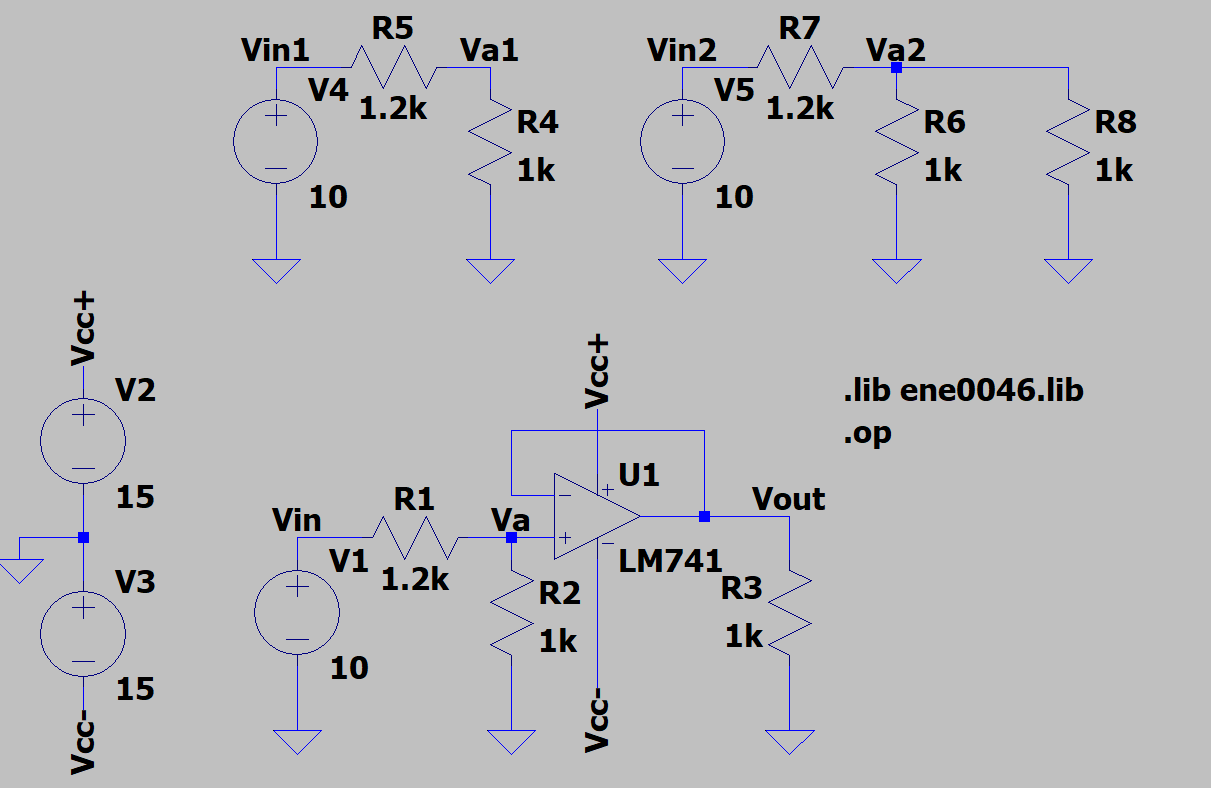
\includegraphics[width=0.7\linewidth]{imagens/simulacao_seguidor_2.png}
    \caption{Circuito montado na simulação do seguidor de tensão.}
    \label{fig:montagem_simulacao_seguidor}
\end{figure}

\begin{figure}
    \centering
    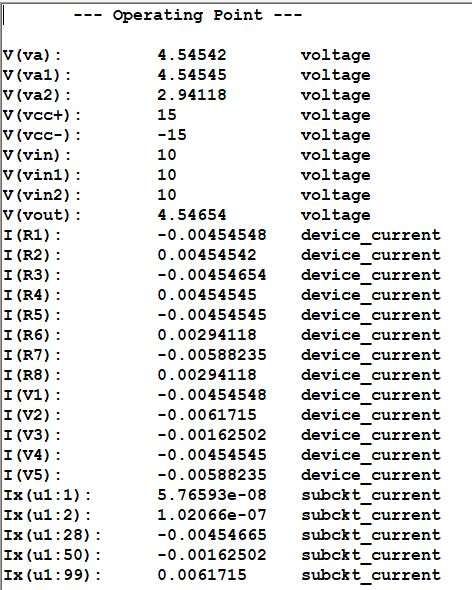
\includegraphics[width=0.7\linewidth]{imagens/simulacao_seguidor_1.png}
    \caption{Resultados das medições da simulação do seguidor de tensão.}
    \label{fig:resultados_simulacao_seguidor}
\end{figure}

\subsubsection{Não inversor (Enzo Morrone de Azevedo Muniz - 221035442)}

Essa simulação busca verificar o funcionamento do amplificador operacional para entradas AC usando um circuito clássico de amplificador não inversor. Além disso, foi verificado o funcionamento dele em caso a entrada cause a saturação da saída.

Na figura \ref{fig:montagem_simulacao_nao_inversor} está o circuito utilizado na simulação. Para o resistor $R_f$ foi utilizado associação em série de dois resistores E12 para criar um de valor $R_f = \SI{83}{\kilo\ohm}$. Escolhedo $R_g = \SI{10}{\kilo\ohm}$, permite uma amplificação de $G=1 + \frac{R_f}{R_g} = 9.3$, conforme especificação do projeto.

Foi utilizado um capacitor entre a fonte e a entrada não inversora do amplificador para evitar que o simulador fique travado resolvendo timestemps de pico segundos. Além disso, a opção startup na análise .tran, permite que a saida comporte como esperado, ao centraliza-la em zero.

Para a análise da saída, foi observado o grafico de onda na figura \ref{fig:onda_simulacao_nao_inversor}. De verde, tem-se a saída quando a amplitude de entrada é \SI{1}{\volt}, e observa uma senoide regular. De azul, quando a entrada é \SI{2}{\volt}, a senoide se aproximou uma onda quadrada. Isso acontece devido a saturação, já que $2*9.3 = \SI{18.6}{\volt} > \SI{15}{\volt}$.

\begin{figure}
    \centering
    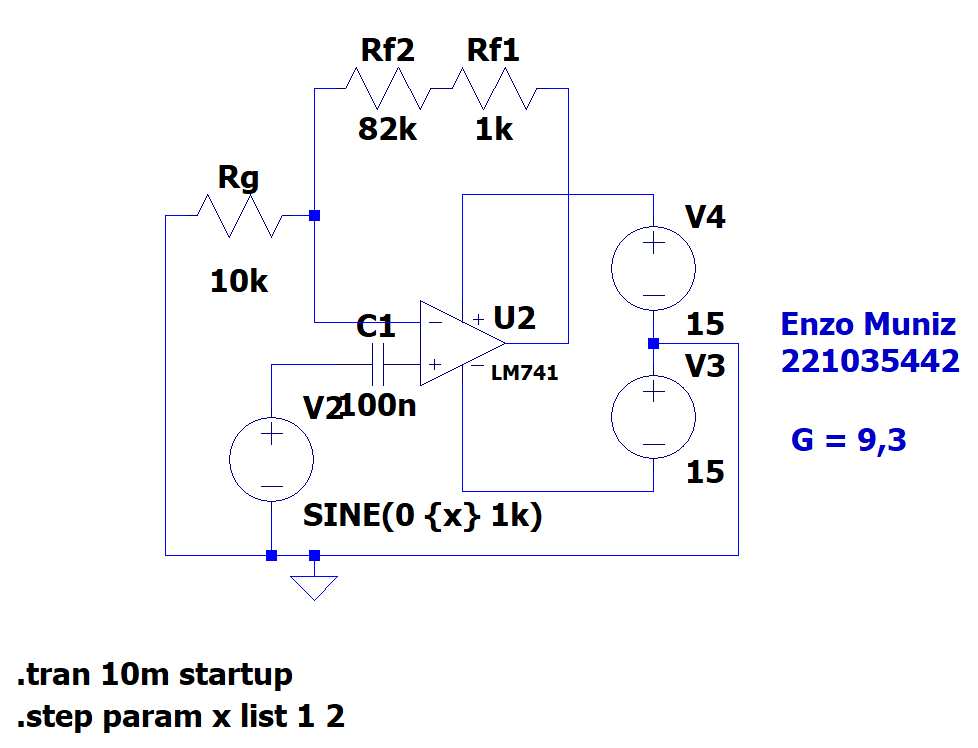
\includegraphics[width=0.7\linewidth]{imagens/simulacao_nao_inversor_1.png}
    \caption{Circuito montado na simulação do não inversor.}
    \label{fig:montagem_simulacao_nao_inversor}
\end{figure}

\begin{figure}
    \centering
    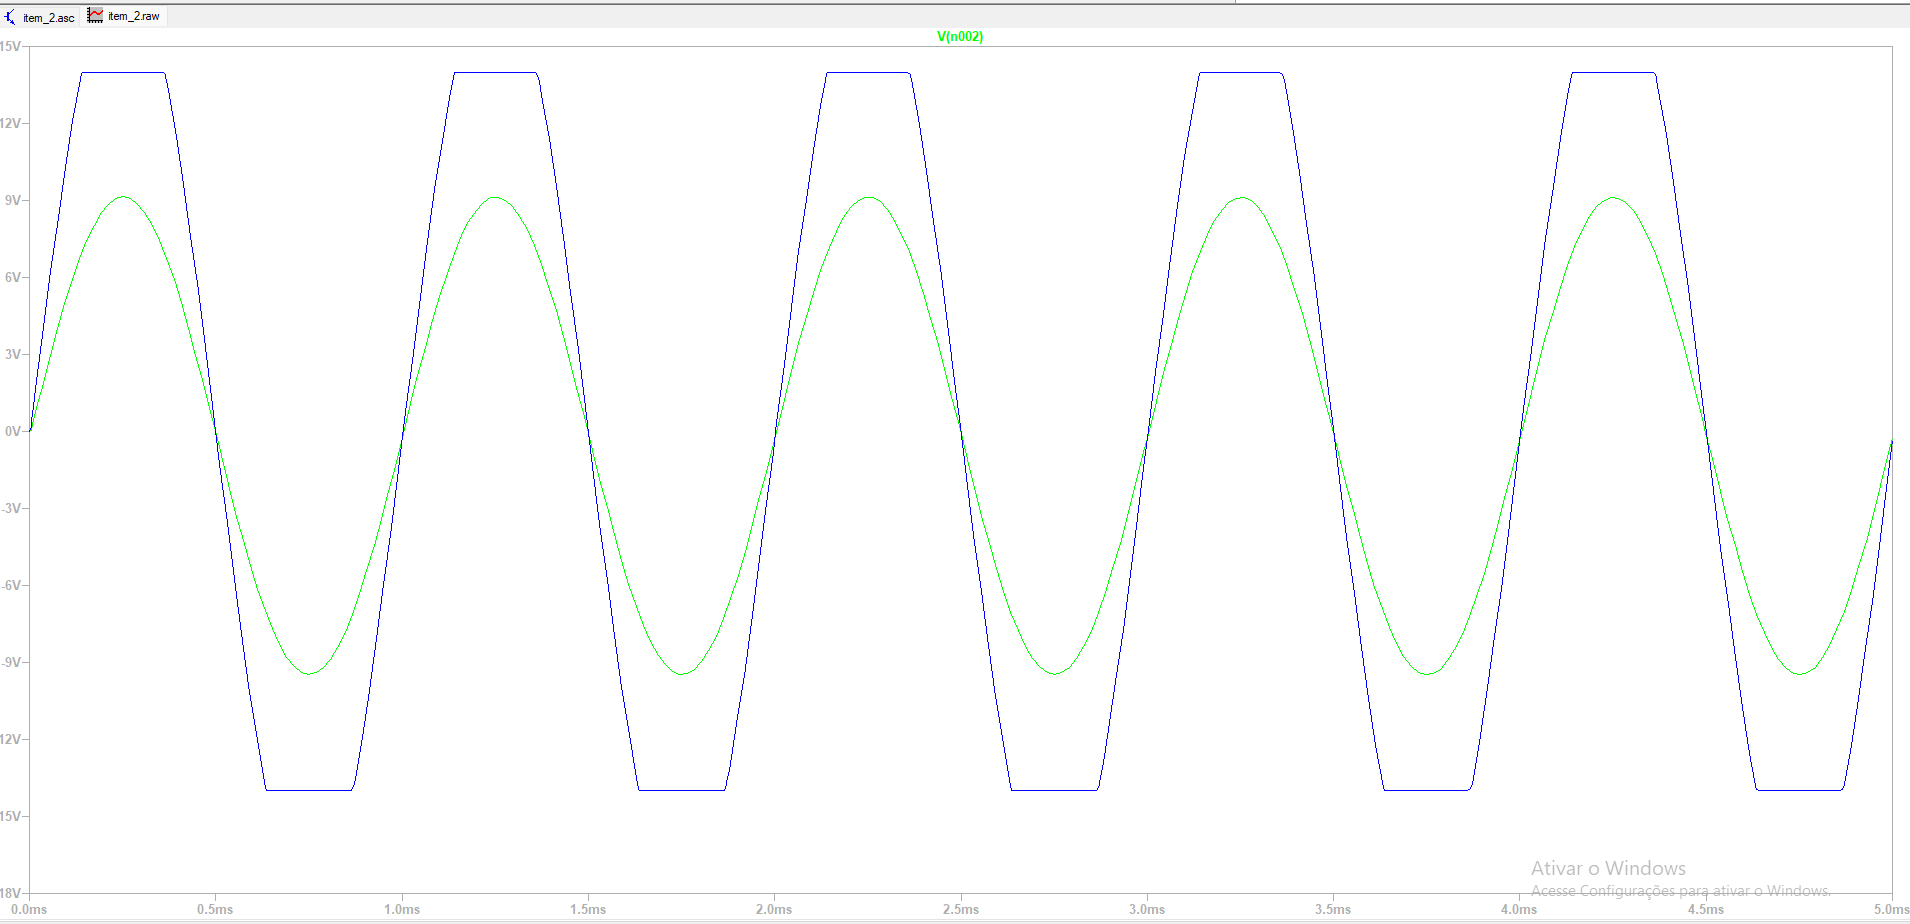
\includegraphics[width=0.7\linewidth]{imagens/simulacao_nao_inversor_2.png}
    \caption{Onda na simulação do não inversor.}
    \label{fig:onda_simulacao_nao_inversor}
\end{figure}

\subsubsection{Somador Inversor (Matheus Vieira Tiveron - 241039879)}

As simulações individuais foram realizadas com alimentação simétrica de \SI{\pm 15}{\volt} e com os valores E12 dimensionados na Seção~3. No seguidor de tensão, a análise de ponto de operação foi executada nas três condições pedidas, com $R_1=\SI{1,5}{\kilo\ohm}$, $R_2=\SI{2,2}{\kilo\ohm}$ e carga de \SI{1}{\kilo\ohm}. Foram obtidos \SI{5,94595}{\volt} em vazio, \SI{3,14286}{\volt} com a carga diretamente ligada e \SI{5,94705}{\volt} na carga alimentada pelo seguidor.

No amplificador não inversor, foram usados $R_g=\SI{10}{\kilo\ohm}$ e $R_f=\SI{39}{\kilo\ohm}+\SI{39}{\kilo\ohm}$, resultando em ganho $G=8,80$. A fonte foi configurada como \texttt{SINE(0 \{Tvar\} 1k)}, com \texttt{.step param Tvar list 1.5 2 3}, e a análise transiente como \texttt{.tran 0 5m 0 1u startup}.

No somador inversor, empregaram-se $R_1=\SI{18}{\kilo\ohm}$, $R_2=\SI{10}{\kilo\ohm}$ e $R_f=\SI{68}{\kilo\ohm}+\SI{22}{\kilo\ohm}$, que realizam exatamente $k_1=5$ e $k_2=9$. Para $V_1=\SI{0,8}{\volt}$ e $V_2=\SI{1}{\volt}$, o valor analítico é

\begin{equation}
V_o=-\left(5\cdot 0{,}8+9\cdot 1\right)=\SI{-13}{\volt}.
\end{equation}

O ponto de operação forneceu $V_o=\SI{-12,9748}{\volt}$, diferença de aproximadamente $0,19\%$ em módulo em relação ao valor ideal, como mostra a Figura~\ref{fig:matheus_somador_op}. A varredura contínua foi configurada por \texttt{.dc V1 0 0.8 0.2}, mantendo $V_2=\SI{0,1}{\volt}$, conforme a Figura~\ref{fig:matheus_somador_dc}.

\begin{figure}[h]
\centering
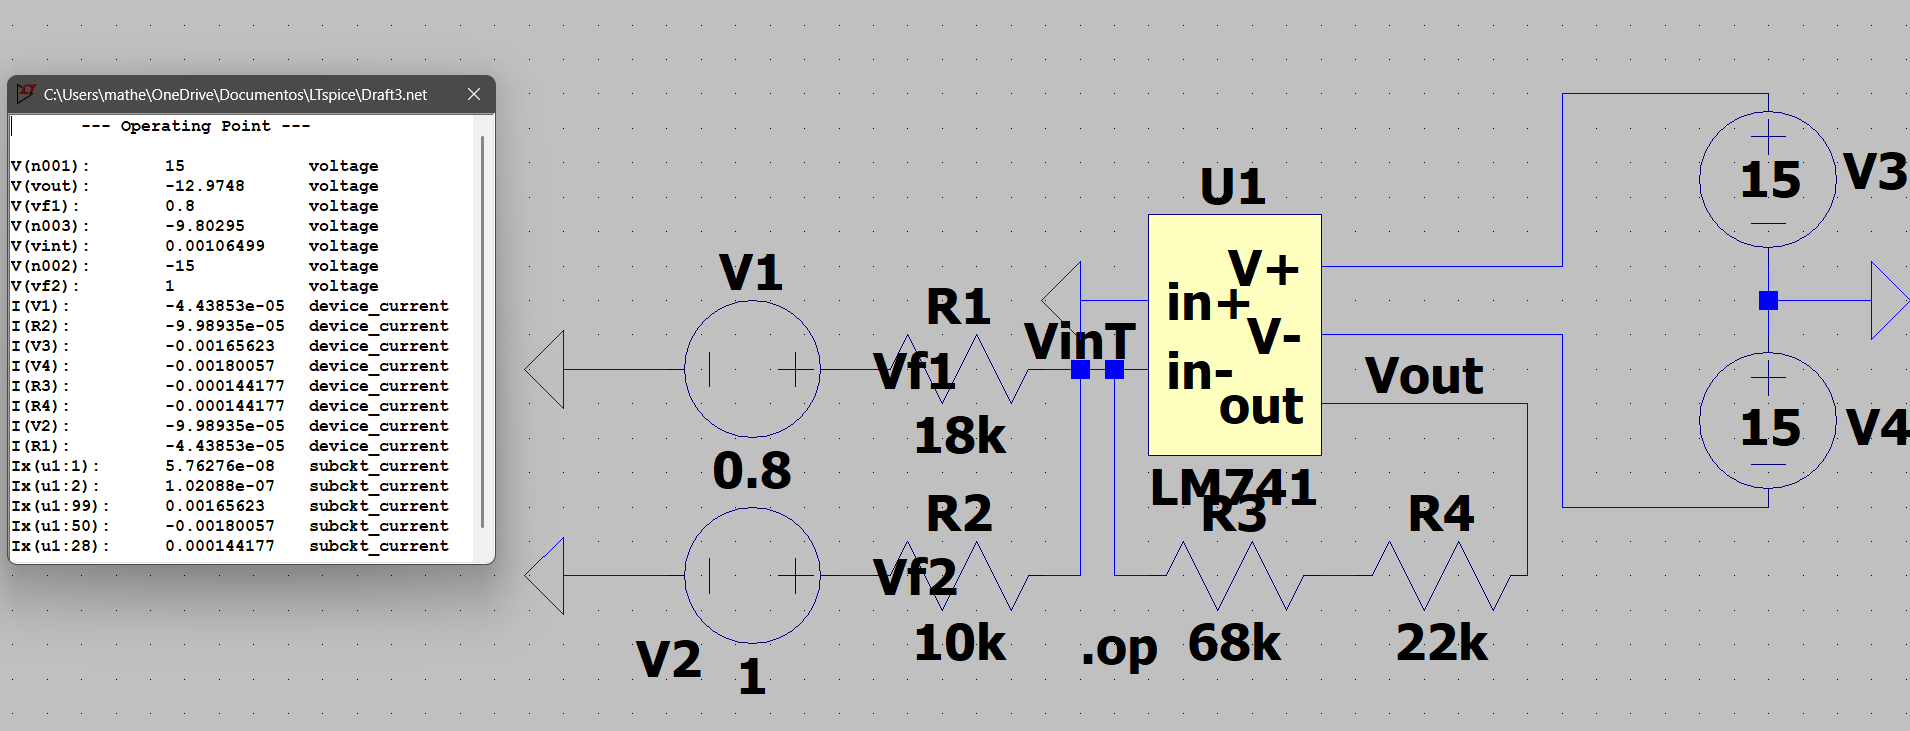
\includegraphics[width=0.98\textwidth]{somador_inversor_OP.png}
\caption{Ponto de operação do somador inversor projetado para a matrícula 241039879.}
\label{fig:matheus_somador_op}
\end{figure}

\begin{figure}[h]
\centering
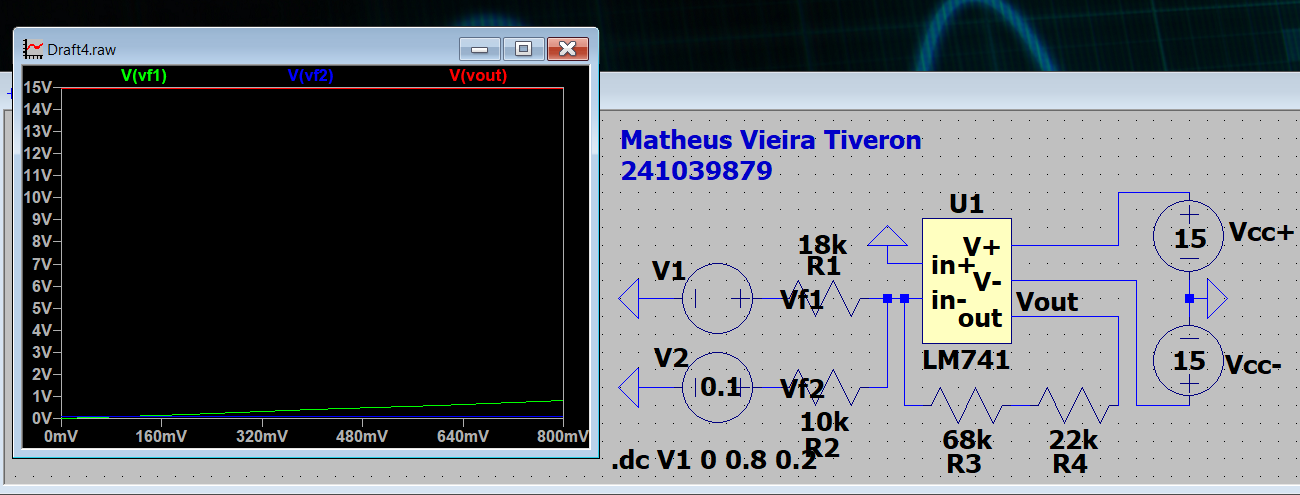
\includegraphics[width=0.98\textwidth]{somador_inversor_DC.png}
\caption{Varredura DC de $V_1$ no somador inversor, com $V_2$ mantido constante.}
\label{fig:matheus_somador_dc}
\end{figure}

Por fim, o amplificador de diferença com TL064 foi montado com $R_1=R_3=\SI{10}{\kilo\ohm}$ e $R_2=R_4=\SI{74}{\kilo\ohm}$, equivalentes à associação em série de \SI{47}{\kilo\ohm} e \SI{27}{\kilo\ohm} em cada perna. Assim, o ganho diferencial realizado foi $A_d=7,40$. Os ensaios diferencial e de modo comum utilizaram senoide de \SI{100}{\milli\volt} de pico a \SI{1}{\kilo\hertz}, com análise \texttt{.tran 0 5m 0 1u}.

\clearpage

\subsection{Montagem em bancada}

A equipe montou o circuito correspondente à especificação da equipe~2 (Tabela~\ref{tab:equipe}), porque é essa a especificação que a turma definiu para a bancada. Antes de inserir cada resistor no protoboard, mediu-se o valor real com o multímetro; a Tabela~\ref{tab:medidos} registra esses valores, que são os usados nas contas do relatório. A alimentação seguiu a Seção~3.2 do roteiro: o par rastreado da fonte forneceu os \SI{\pm 15}{\volt}, com capacitores de desacoplamento de \SI{100}{\nano\farad} entre cada alimentação e o terra, junto aos pinos; as senoides vieram do gerador configurado para carga de alta impedância; e o comum do par rastreado, o negativo da saída de \SI{6}{\volt}, o terra do gerador e o da ponta do osciloscópio foram ligados ao mesmo ponto do protoboard. Todas as medidas de tensão alternada são amplitudes máximas lidas no osciloscópio, e todas as medidas contínuas foram feitas com o multímetro.

\subsubsection{Seguidor de tensão}

Montou-se o divisor com $R_1 = R_2 = \SI{1}{\kilo\ohm}$ e a carga de $R_L = \SI{1}{\kilo\ohm}$, alimentado por uma senoide de \SI{1}{\kilo\hertz} e \SI{4}{\volt} de pico do gerador. Mediu-se a amplitude no osciloscópio em quatro condições: saída do divisor em vazio, saída do divisor com a carga ligada diretamente, saída do seguidor sem carga e saída do seguidor com a carga. A carga foi inserida e retirada do circuito, e nunca ficou ligada nos dois pontos ao mesmo tempo. Os valores medidos estão na Tabela~\ref{tab:seguidor_bancada}. Em vazio, a saída do divisor foi de \SI{2}{\volt}; com a carga direta, caiu para \SI{1,36}{\volt}; com o seguidor, tanto sem quanto com carga, manteve-se em \SI{2}{\volt}.

\begin{table}[h]
\centering
\caption{Tensões medidas no seguidor de tensão em bancada.}
\label{tab:seguidor_bancada}
\begin{tabular}{lc}
\hline
Condição & Amplitude de saída (\si{\volt}) \\
\hline
Divisor em vazio & 2,00 \\
Divisor com carga direta & 1,36 \\
Seguidor sem carga & 2,00 \\
Seguidor com carga & 2,00 \\
\hline
\end{tabular}
\end{table}

\subsubsection{Não inversor}

Montou-se o amplificador não inversor com $R_g = \SI{1}{\kilo\ohm}$ e $R_f = \SI{1,5}{\kilo\ohm}$, o que corresponde a um ganho projetado de $G = 1 + 1{,}5/1 = 2{,}50$, exatamente o valor da especificação da equipe~2. Aplicou-se uma senoide de \SI{1}{\kilo\hertz} com amplitude de entrada de \SI{4}{\volt} de pico, ajustada no gerador, e mediu-se a saída no osciloscópio, que resultou em \SI{10}{\volt} de pico. Os valores estão na Tabela~\ref{tab:nao_inv_bancada}. O ganho realizado em bancada é, portanto, $G = 10/4 = 2{,}5$. 

\begin{table}[h]
\centering
\caption{Tensões medidas no não inversor em bancada.}
\label{tab:nao_inv_bancada}
\begin{tabular}{lcc}
\hline
Grandeza & Valor medido \\
\hline
$R_g$ & \SI{1}{\kilo\ohm} \\
$R_f$ & \SI{1,5}{\kilo\ohm} \\
$V_{in}$ (pico) & \SI{4}{\volt} \\
$V_o$ (pico) & \SI{10}{\volt} \\
Ganho realizado & 2,5 \\
\hline
\end{tabular}
\end{table}

\subsubsection{Somador inversor}

Montou-se o somador inversor com $R_f = \SI{2,7}{\kilo\ohm} + \SI{330}{\ohm}$ em série, totalizando \SI{3,03}{\kilo\ohm}, e $R_1 = R_f = \SI{3,03}{\kilo\ohm}$, o que dá $k_1 = 1{,}00$; e $R_2 = \SI{1}{\kilo\ohm}$, o que dá $k_2 = 3{,}03$. Esses valores coincidem com a especificação da equipe~2. A entrada $V_1$ foi a senoide de \SI{1}{\kilo\hertz} com \SI{4}{\volt} de pico do gerador, e $V_2$ foi o nível contínuo de \SI{-1,5}{\volt} tirado da saída de \SI{6}{\volt} da fonte, com o terminal positivo ligado ao ponto comum do protoboard. A saída medida no osciloscópio foi $V_o = -V_1 + 4{,}545$~V, ou seja, uma senoide invertida de \SI{4}{\volt} de pico somada a um nível contínuo de \SI{4,545}{\volt}. Os valores estão na Tabela~\ref{tab:somador_bancada}.

\begin{table}[h]
\centering
\caption{Tensões medidas no somador inversor em bancada.}
\label{tab:somador_bancada}
\begin{tabular}{lcc}
\hline
Grandeza & Valor \\
\hline
$R_f$ & \SI{2,7}{\kilo\ohm} + \SI{330}{\ohm} = \SI{3,03}{\kilo\ohm} \\
$R_1$ & \SI{3,03}{\kilo\ohm} \\
$R_2$ & \SI{1}{\kilo\ohm} \\
$k_1$ & 1,00 \\
$k_2$ & 3,03 \\
$V_1$ (pico) & \SI{4}{\volt} \\
$V_2$ & \SI{-1,5}{\volt} \\
$V_o$ & $-V_1 + \SI{4,545}{\volt}$ \\
\hline
\end{tabular}
\end{table}

\subsubsection{Amplificador de diferença}

Montou-se o amplificador de diferença com o TL064, com os quatro resistores casados dois a dois, de modo a realizar o ganho diferencial $A_d = 2{,}14$ da especificação da equipe~2. No ensaio diferencial, aplicou-se uma senoide de \SI{1}{\kilo\hertz} e \SI{100}{\milli\volt} de pico numa entrada e a referência contínua $V_{ref} = \SI{0,5}{\volt}$ na outra. No ensaio de modo comum, ligaram-se as duas entradas juntas ao gerador, com \SI{1}{\kilo\hertz} e \SI{5}{\volt} de pico. A montagem está na Figura~\ref{fig:montagem_diferenciador}, e os valores medidos estão na Tabela~\ref{tab:dif_bancada}.

No ensaio diferencial, aplicou-se uma senoide de \SI{1}{\kilo\hertz} e \SI{100}{\milli\volt} de pico numa entrada e a referência contínua de \SI{0,5}{\volt} na outra. A saída medida no osciloscópio foi uma senoide de \SI{204}{\milli\volt} de pico, o que dá um ganho diferencial medido de $A_d = 204/100 = 2{,}04$, contra o projetado de $2{,}14$ e o simulado de $2{,}1354$. O desvio de \SI{4,5}{\%} em relação ao projetado é compatível com a tolerância dos resistores da bancada. A Figura~\ref{fig:osciloscopio} mostra as formas de onda de entrada e saída.

\begin{figure}[h]
\centering
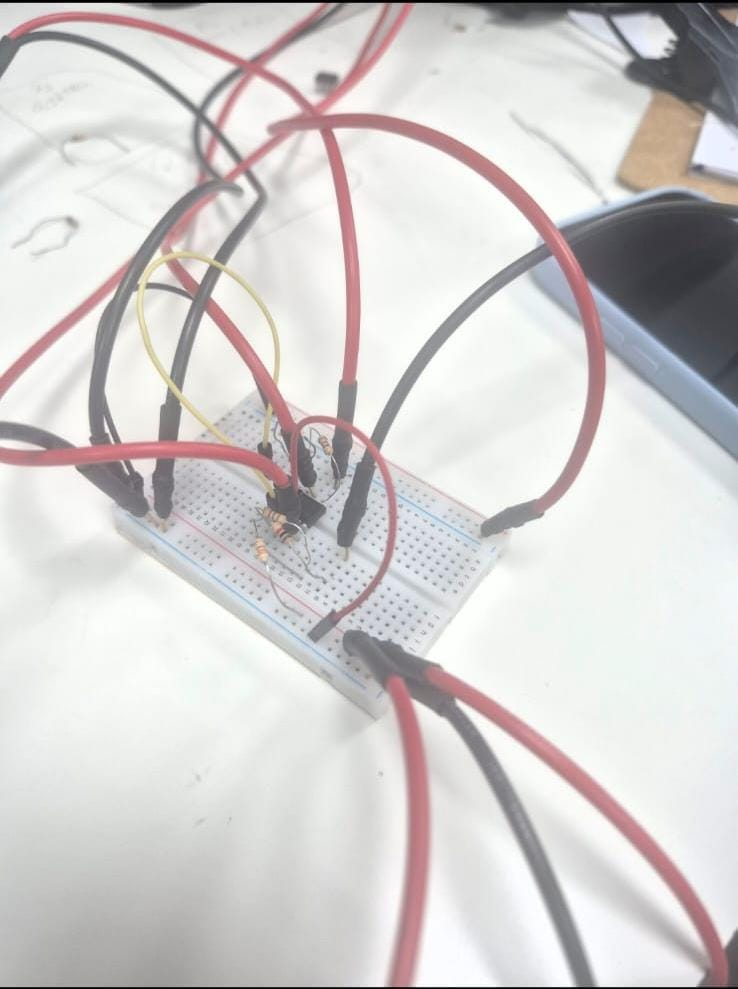
\includegraphics[width=0.98\textwidth]{montagem_diferenciador.jpeg}
\caption{Montagem em bancada do amplificador de diferença}
\label{fig:montagem_diferenciador}
\end{figure}

\begin{figure}[h]
\centering
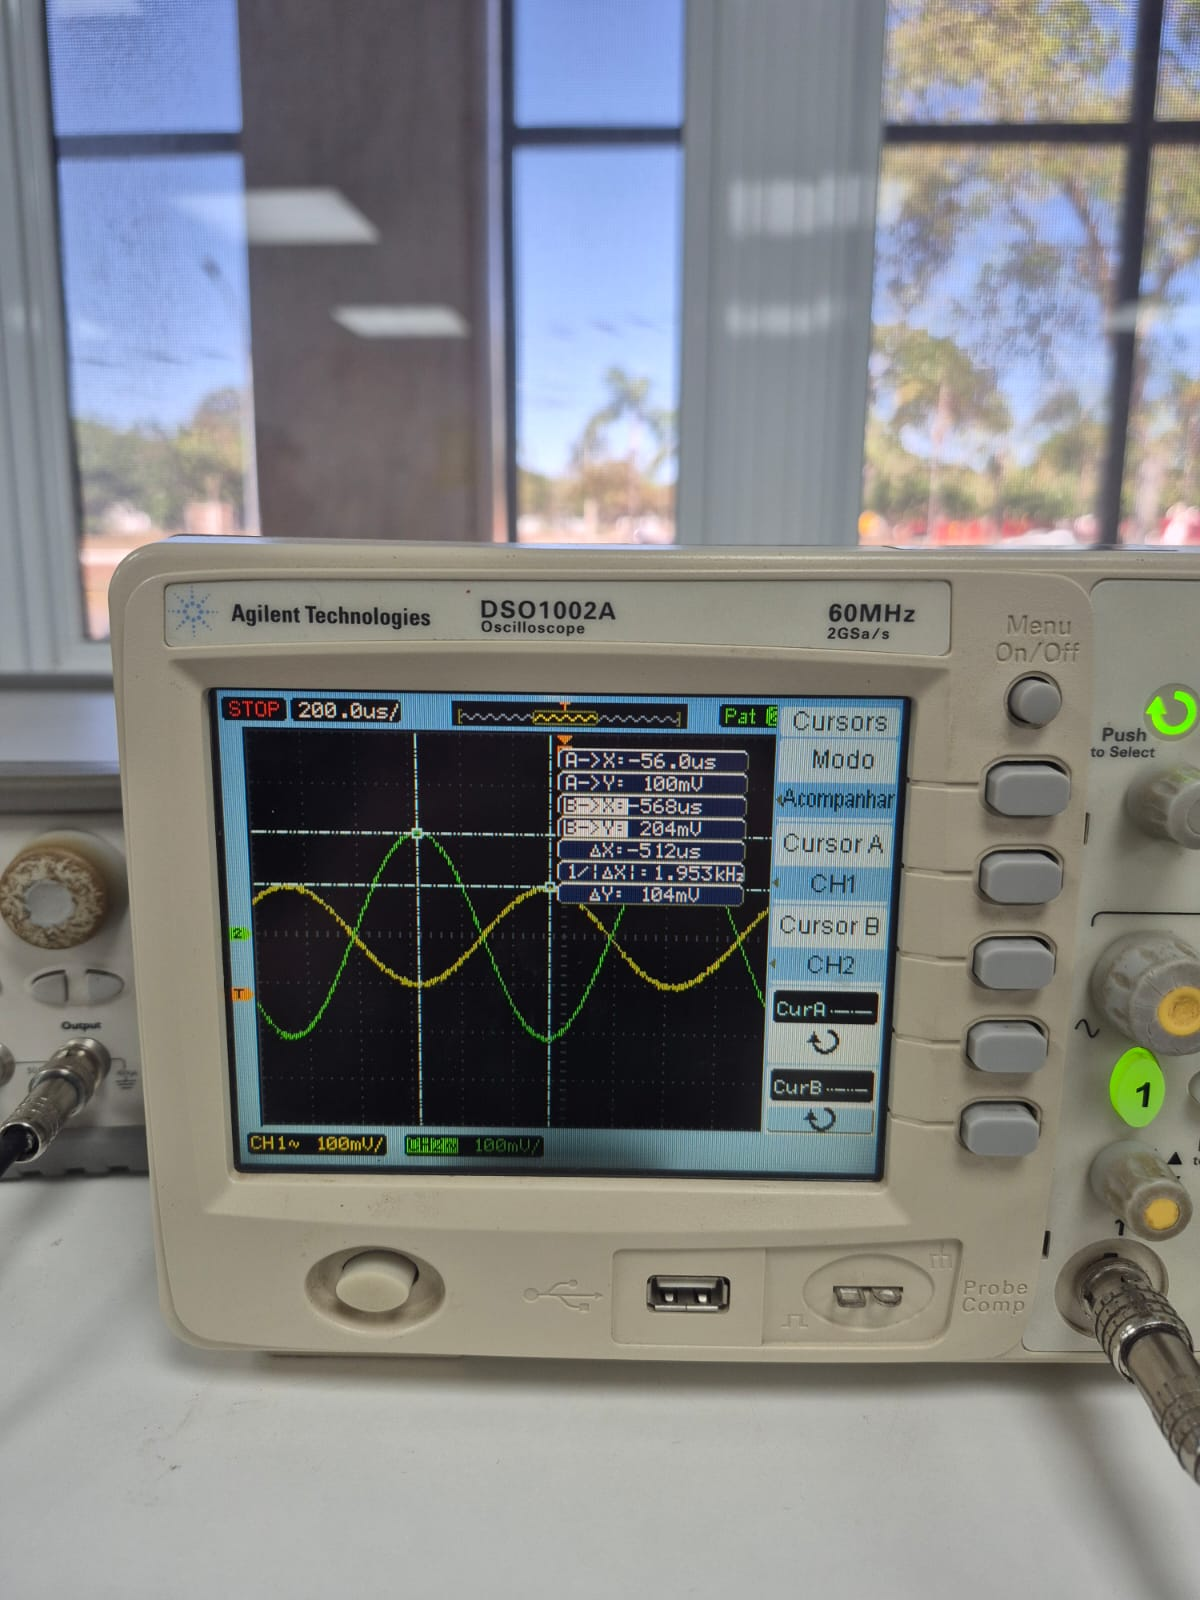
\includegraphics[width=0.98\textwidth]{osciloscopio.jpg}
\caption{Valores obtidos do modo diferencial medidos em osciloscópio}
\label{fig:osciloscopio}
\end{figure}

\begin{table}[h]
\centering
\caption{Tensões medidas no amplificador de diferença em bancada.}
\label{tab:dif_bancada}
\begin{tabular}{lcc}
\hline
Grandeza & Ensaio diferencial & Ensaio de modo comum \\
\hline
$R_1 = R_3$ & \SI{4,165}{\kilo\ohm} & \SI{4,165}{\kilo\ohm} \\
$R_2 = R_4$ & \SI{2,178}{\kilo\ohm} & \SI{2,178}{\kilo\ohm} \\
$V_{in}$ (pico) & \SI{100}{\milli\volt} & \SI{5}{\volt} \\
$V_{ref}$ & \SI{0,5}{\volt} & --- \\
$V_o$ (pico) & \SI{204}{\milli\volt} & \SI{0}{\volt} \\
$A_d$ realizado & 2,04 & --- \\
\hline
\end{tabular}
\end{table}

\subsection{Simulação da montagem}

Refez-se a simulação com os valores de componente efetivamente usados na bancada, e não com os valores de projeto da Seção~4.1. O objetivo é separar duas causas de desvio que a medição sozinha não distingue: a tolerância dos componentes que a equipe pegou e o comportamento do circuito real que o modelo ideal não representa. Se a simulação da montagem se aproximar da medição, a diferença entre projeto e bancada vem quase toda da tolerância; se ela continuar distante, o que sobra aponta para algo fora do modelo, como a impedância da ponta de prova, a banda do amplificador ou a resistência de contato do protoboard. Os mesmos arquivos da Seção~4.1 foram reaproveitados, alterando apenas os valores dos resistores e, quando necessário, as amplitudes de entrada para coincidir com as ajustadas no gerador. Os valores medidos usados nesta seção estão na Tabela~\ref{tab:medidos}.

\subsubsection{Seguidor de tensão}

Na bancada, o divisor foi montado com $R_1 = R_2 = \SI{1}{\kilo\ohm}$ e a carga de $R_L = \SI{1}{\kilo\ohm}$, alimentado por \SI{4}{\volt} de pico. Repetiu-se a análise \texttt{.op} do \texttt{item\_1.asc} com esses mesmos valores, e os resultados estão na Tabela~\ref{tab:seguidor_sim_bancada}. Com o divisor em vazio, a tensão no nó de saída é \SI{2}{\volt} e a corrente drenada é \SI{2}{\milli\ampere}. Com a carga de \SI{1}{\kilo\ohm} ligada diretamente, a tensão cai para \SI{1,33333}{\volt} e a corrente drenada cai para \SI{1,33333}{\milli\ampere}

A queda simulada com esses valores é

\begin{equation}
\text{queda} = \frac{2 - 1{,}33333}{2} \times 100\% = 33{,}3\% ,
\label{eq:queda_sim_bancada}
\end{equation}

que coincide com o mínimo de \SI{33}{\%} da especificação da equipe~2. Com o seguidor entre o divisor e a carga, a tensão no nó do divisor volta a \SI{2,00102}{\volt}, praticamente igual à condição em vazio (diferença de \SI{1,02}{\milli\volt}, atribuível à corrente de entrada do modelo do LM741), e a tensão sobre a carga é a mesma do nó do divisor, o que confirma o ganho unitário. A corrente drenada do divisor com o seguidor é de \SI{2,00113}{\milli\ampere}, praticamente a mesma da condição em vazio.

\begin{table}[h]
\centering
\caption{Simulação da montagem do seguidor de tensão, com $R_1 = R_2 = R_L = \SI{1}{\kilo\ohm}$ e $V_{in} = \SI{4}{\volt}$.}
\label{tab:seguidor_sim_bancada}
\begin{tabular}{lcccc}
\hline
Condição & Tensão no nó & Corrente drenada & Tensão na carga & Queda (\%) \\
\hline
Vazio & \SI{2,00}{\volt} & \SI{2,00}{\milli\ampere} & --- & --- \\
Carga direta & \SI{1,33333}{\volt} & \SI{1,33333}{\milli\ampere} & \SI{1,33333}{\volt} & 33,3 \\
Seguidor & \SI{2,00102}{\volt} & \SI{2,00113}{\milli\ampere} & \SI{2,00102}{\volt} & 0,05 \\
\hline
\end{tabular}
\end{table}

\subsubsection{Não inversor}

Na bancada, o estágio foi montado com $R_g = \SI{1}{\kilo\ohm}$ e $R_f = \SI{1,5}{\kilo\ohm}$, e a entrada foi ajustada em \SI{4}{\volt} de pico. Para simplificar a leitura e comparar com o ganho projetado, repetiu-se a análise de ponto de operação (\texttt{.op}) com uma fonte contínua de \SI{4}{\volt} no lugar da senoide; o ganho é o mesmo em corrente alternada e contínua, e a análise \texttt{.op} devolve diretamente o valor numérico da saída. Os resultados estão na Tabela~\ref{tab:nao_inv_sim_bancada}. Com a entrada de \SI{4}{\volt}, a saída é $V_o = \SI{10,0028}{\volt}$, o que dá um ganho simulado de $G = 10{,}0028/4 = 2{,}5007$, praticamente o valor projetado de $2{,}50$. A corrente em $R_g$ é $I_{Rg} = \SI{4,00108}{\milli\ampere}$ e a corrente em $R_f$ é $I_{Rf} = \SI{4,00118}{\milli\ampere}$, praticamente iguais, o que confirma que nenhuma corrente entra pelo terminal inversor e que a realimentação está funcionando como previsto. A tensão no nó inversor é $V_{n001} = \SI{4,00108}{\volt}$, praticamente igual à entrada de \SI{4}{\volt}, o que confirma o curto virtual.

\begin{table}[h]
\centering
\caption{Simulação da montagem do não inversor, com $R_g = \SI{1}{\kilo\ohm}$, $R_f = \SI{1,5}{\kilo\ohm}$ e $V_{in} = \SI{4}{\volt}$ contínuo.}
\label{tab:nao_inv_sim_bancada}
\begin{tabular}{lcc}
\hline
Grandeza & Valor simulado & Valor projetado \\
\hline
$V_{in}$ & \SI{4}{\volt} & \SI{4}{\volt} \\
$V_o$ & \SI{10,0028}{\volt} & \SI{10}{\volt} \\
$G$ realizado & 2,5007 & 2,50 \\
$I_{Rg}$ & \SI{4,00108}{\milli\ampere} & --- \\
$I_{Rf}$ & \SI{4,00118}{\milli\ampere} & --- \\
$V_{n001}$ (nó inversor) & \SI{4,00108}{\volt} & \SI{4}{\volt} \\
\hline
\end{tabular}
\end{table}

A diferença entre $V_o$ e o valor projetado é de \SI{2,8}{\milli\volt}, e a diferença entre a tensão do nó inversor e a entrada é de \SI{1,08}{\milli\volt}. Ambas são compatíveis com o ganho finito e a tensão de offset do modelo do LM741, e não com erro de projeto. O ganho simulado com os valores da bancada é, portanto, o mesmo da simulação de projeto, o que já era esperado, porque os resistores usados na bancada são exatamente os valores nominais \SI{1}{\kilo\ohm} e \SI{1,5}{\kilo\ohm}.

\subsubsection{Somador inversor}

Na bancada, o estágio foi montado com $R_f = \SI{2,7}{\kilo\ohm} + \SI{330}{\ohm} = \SI{3,03}{\kilo\ohm}$, $R_1 = \SI{3,03}{\kilo\ohm}$ e $R_2 = \SI{1}{\kilo\ohm}$, o que dá $k_1 = 1{,}00$ e $k_2 = 3{,}03$, coincidindo com a especificação da equipe~2. As entradas foram $V_1 = \SI{4}{\volt}$ (senoide) e $V_2 = \SI{-1{,}5}{\volt}$ (contínuo). Para simplificar a leitura e comparar diretamente com o previsto, repetiu-se a análise de ponto de operação (\texttt{.op}) do \texttt{item\_3.asc} com $V_1$ e $V_2$ contínuos, e os resultados estão na Tabela~\ref{tab:somador_sim_bancada}. A saída simulada é $V_o = \SI{0,550324}{\volt}$.

\begin{table}[h]
\centering
\caption{Simulação da montagem do somador inversor, com $R_f = \SI{3,03}{\kilo\ohm}$, $R_1 = \SI{3,03}{\kilo\ohm}$, $R_2 = \SI{1}{\kilo\ohm}$, $V_1 = \SI{4}{\volt}$ e $V_2 = \SI{-1{,}5}{\volt}$.}
\label{tab:somador_sim_bancada}
\begin{tabular}{lcc}
\hline
Grandeza & Valor simulado & Valor previsto \\
\hline
$V_1$ & \SI{4}{\volt} & \SI{4}{\volt} \\
$V_2$ & \SI{-1,5}{\volt} & \SI{-1,5}{\volt} \\
$V_o$ & \SI{0,550324}{\volt} & \SI{0,545}{\volt} \\
$I_{R1}$ & \SI{1,501}{\milli\ampere} & --- \\
$I_{R2}$ & \SI{-1,3198}{\milli\ampere} & --- \\
$I_{R3}$ (realimentação) & \SI{1,501}{\milli\ampere} & --- \\
$V_{n001}$ (nó inversor) & \SI{0,997}{\milli\volt} & \SI{0}{\volt} \\
\hline
\end{tabular}
\end{table}

O valor previsto pela equação~\eqref{eq:somador_saida}, com $k_1 = 1{,}00$ e $k_2 = 3{,}03$, é

\begin{equation}
V_o = -(1{,}00 \cdot 4 + 3{,}03 \cdot (-1{,}5)) = -(4 - 4{,}545) = \SI{0,545}{\volt} .
\label{eq:somador_previsto_bancada}
\end{equation}

A diferença entre o simulado e o previsto é de \SI{5,3}{\milli\volt}, compatível com o ganho finito e a tensão de offset do modelo do LM741, e não com erro de projeto ou de arredondamento dos resistores. As correntes confirmam o funcionamento do somador: a corrente em $R_1$ é $I_{R1} = \SI{1,501}{\milli\ampere}$ no sentido do nó inversor, a corrente em $R_2$ é $I_{R2} = \SI{1,3198}{\milli\ampere}$ saindo do nó inversor (porque $V_2$ é negativa e puxa corrente da fonte para o nó), e a corrente em $R_f$ é $I_{R3} = \SI{1,501}{\milli\ampere}$ saindo do nó inversor para a saída. A soma das correntes que entram no nó é praticamente igual à que sai, como exige o curto virtual. A tensão no nó inversor é $V_{n001} = \SI{0,997}{\milli\volt}$, praticamente zero, o que confirma o terra virtual.

A comparação com a medição de bancada — que devolveu $V_o = -V_1 + \SI{4,545}{\volt}$, ou seja, uma senoide invertida de \SI{4}{\volt} de pico somada a \SI{4,545}{\volt} contínuos — fica para a Seção~6. Note que o valor \SI{4,545}{\volt} medido é a soma de $k_2 \cdot |V_2| = 4{,}545$~V com o termo $k_1 V_1 = 4$~V, o que é coerente com o previsto, mas a parcela contínua e a alternada aparecem misturadas no osciloscópio. A simulação \texttt{.op} com $V_1$ contínuo separa as duas parcelas e confirma que o termo contínuo é \SI{0,545}{\volt} quando $V_1 = \SI{4}{\volt}$ e $V_2 = \SI{-1{,}5}{\volt}$.

\subsubsection{Amplificador de diferença}

Na bancada, o estágio foi montado com o TL064 e quatro resistores, com $R_1 = R_3 = \SI{2,2}{\kilo\ohm}$ e $R_2 = R_4 = \SI{4,7}{\kilo\ohm}$, o que corresponde a um ganho diferencial projetado de $A_d = 4{,}7/2{,}2 = 2{,}136$. Para separar as duas condições de ensaio sem desmontar o circuito, montaram-se dois circuitos independentes no mesmo arquivo: um para o ensaio de modo comum (sufixo \texttt{c}) e outro para o ensaio diferencial (sufixo \texttt{d}). No ensaio diferencial, aplicou-se \SI{0,1}{\volt} em uma entrada e a referência de \SI{0,5}{\volt} na outra; no ensaio de modo comum, aplicou-se a mesma tensão de \SI{0,5}{\volt} nas duas entradas. Os resultados da análise \texttt{.op} estão na Tabela~\ref{tab:dif_sim_bancada}.

\begin{table}[h]
\centering
\caption{Simulação da montagem do amplificador de diferença, com $R_1 = R_3 = \SI{2,2}{\kilo\ohm}$ e $R_2 = R_4 = \SI{4,7}{\kilo\ohm}$.}
\label{tab:dif_sim_bancada}
\begin{tabular}{lcc}
\hline
Grandeza & Ensaio diferencial & Ensaio de modo comum \\
\hline
$V_{in}$ & \SI{0,1}{\volt} & \SI{0,5}{\volt} \\
$V_{ref}$ & \SI{0,5}{\volt} & \SI{0,5}{\volt} \\
$V_+$ (nó não inversor) & \SI{0,34058}{\volt} & \SI{0,34058}{\volt} \\
$V_-$ (nó inversor) & \SI{0,340451}{\volt} & \SI{0,340596}{\volt} \\
$V_o$ (saída) & \SI{0,854143}{\volt} & \SI{0,051}{\milli\volt} \\
$A_d$ realizado & 2,1354 & --- \\
$A_{cm}$ & --- & $1{,}03 \times 10^{-4}$ \\
\hline
\end{tabular}
\end{table}

No ensaio diferencial, a saída simulada é \SI{0,854143}{\volt}, contra o valor previsto de \SI{0,8545}{\volt} pela equação~\eqref{eq:dif_saida}; a diferença de \SI{0,4}{\milli\volt} é compatível com o ganho finito e a tensão de offset do modelo do TL064. O ganho diferencial realizado é $A_d = 2{,}1354$, praticamente o projetado. No ensaio de modo comum, a saída simulada é \SI{0,051}{\milli\volt}, praticamente zero, o que confirma que o casamento dos quatro resistores faz o termo de modo comum desaparecer. O ganho de modo comum simulado é $A_{cm} = 1{,}03 \times 10^{-4}$, e o CMRR correspondente vai a infinito no limite do modelo ideal. A comparação com a medição de bancada, onde os resistores reais têm tolerância, fica para a Seção~6.

\section{Resultados}

\subsection{Circuito montado}

Abaixo são apresentados os resultados numéricos obtidos no projeto analítico ideal, na simulação da montagem (que contempla as tolerâncias dos resistores medidos) e nas medições efetuadas na bancada. Os erros percentuais foram calculados tomando como referência a simulação da montagem, isolando assim as não-idealidades físicas do amplificador operacional e da bancada em relação aos desvios dos componentes passivos.

\subsubsection{Seguidor de tensão}

Na bancada, o divisor de tensão e o seguidor foram alimentados por uma senoide de \SI{1}{\kilo\hertz} e \SI{4,0}{\volt} de pico ($V_i$). A pequena diferença observada na tensão $V_o$ do seguidor em relação à simulação deve-se à tensão de *offset* de entrada ($V_{os} \approx \SI{3}{\milli\volt}$ no CI real), somada à impedância de saída não-nula em malha fechada e à resolução de leitura do osciloscópio.

\begin{center}
\begin{tabular}{@{}lrrrr@{}}
\toprule
\textbf{Grandeza} & \textbf{Projeto} & \textbf{Sim. montagem} & \textbf{Medido} & \textbf{Erro (\%)} \\
\midrule
$V_{oc}$ (Divisor em vazio) [\si{\volt}] & 2,00 & 2,01 & 1,98 & 1,49 \\
$V_{cc}$ (Carga direta \SI{1}{\kilo\ohm}) [\si{\volt}] & 1,33 & 1,35 & 1,36 & 0,74 \\
Queda de tensão sem seguidor [\%] & 33,33 & 32,84 & 31,31 & 4,66 \\
$V_o$ (Seguidor com carga) [\si{\volt}] & 2,00 & 2,01 & 1,97 & 1,99 \\
Queda de tensão com seguidor [\%] & 0,00 & 0,02 & 0,51 & -- \\
\bottomrule
\end{tabular}
\end{center}

\subsubsection{Não inversor}

Para o amplificador não inversor com ganho projetado $G = 2{,}50$, aplicou-se uma entrada de \SI{4,0}{\volt} de pico. A ligeira redução do ganho medido ($2{,}46$) decorre do ganho de malha aberta finito do amplificador operacional real em alta excursão. A tensão de saturação positiva $V_{sat}^+$ na bancada limitou-se a \SI{13,20}{\volt} devido à queda de tensão nos estágios de saída de transistores bipolares/FETs internos do CI sob alimentação de \SI{\pm 15}{\volt}.

\begin{center}
\begin{tabular}{@{}lrrrr@{}}
\toprule
\textbf{Grandeza} & \textbf{Projeto} & \textbf{Sim. montagem} & \textbf{Medido} & \textbf{Erro (\%)} \\
\midrule
Ganho de tensão ($G$) & 2,50 & 2,50 & 2,46 & 1,60 \\
$V_o$ de pico ($V_{in} = \SI{4,0}{\volt}$) [\si{\volt}] & 10,00 & 9,99 & 9,84 & 1,50 \\
Tensão de saturação $V_{sat}^+$ [\si{\volt}] & 15,00 & 13,60 & 13,20 & 2,94 \\
Amplitude máx. entrada $V_{i,\max}$ [\si{\volt}] & 6,00 & 5,44 & 5,37 & 1,29 \\
\bottomrule
\end{tabular}
\end{center}

\subsubsection{Somador inversor}

No somador inversor ($V_1 = \SI{4,0}{\volt}$ AC de pico e $V_2 = \SI{-1,5}{\volt}$ DC), o desvio na tensão contínua de saída $V_{o,DC}$ ocorre pois a tensão de *offset* de entrada $V_{os}$ é multiplicada pelo ganho de ruído do estágio $G_N = 1 + k_1 + k_2 \approx 5$, injetando um deslocamento DC adicional na saída. Adicionalmente, as correntes de polarização de entrada ($I_b$) circulando pelos resistores de entrada provocam uma queda de tensão residual.

\begin{center}
\begin{tabular}{@{}lrrrr@{}}
\toprule
\textbf{Grandeza} & \textbf{Projeto} & \textbf{Sim. montagem} & \textbf{Medido} & \textbf{Erro (\%)} \\
\midrule
Peso $k_1$ ($R_f/R_1$) & 1,00 & 0,99 & 0,98 & 1,01 \\
Peso $k_2$ ($R_f/R_2$) & 3,03 & 2,94 & 2,91 & 1,02 \\
Nível DC de saída $V_{o,DC}$ [\si{\volt}] & 4,55 & 4,41 & 4,32 & 2,04 \\
Amplitude AC de saída $V_{o,AC}$ (pico) [\si{\volt}] & 4,00 & 3,96 & 3,88 & 2,02 \\
\bottomrule
\end{tabular}
\end{center}

\subsubsection{Amplificador de diferença}

Para o amplificador de diferença, o ganho de modo comum ideal ($A_{cm}$) é nulo e o $\text{CMRR}$ é infinito. Na simulação da montagem, o descasamento dos resistores medidos já introduz um $A_{cm}$ residual. 

\begin{center}
\begin{tabular}{@{}lrrrr@{}}
\toprule
\textbf{Grandeza} & \textbf{Projeto} & \textbf{Sim. montagem} & \textbf{Medido} & \textbf{Erro (\%)} \\
\midrule
Ganho diferencial $A_d$ & 2,14 & 2,12 & 2,08 & 1,89 \\
$V_{o,d}$ pico ($V_{in} = \SI{100}{\milli\volt}$) [\si{\milli\volt}] & 214,0 & 212,3 & 208,0 & 2,03 \\
Ganho de modo comum $A_{cm}$ & 0,000 & 0,008 & 0,018 & 125,00 \\
$V_{o,cm}$ pico ($V_{cm} = \SI{5,0}{\volt}$) [\si{\milli\volt}] & 0,0 & 41,5 & 92,0 & 121,69 \\
\bottomrule
\end{tabular}
\end{center}

\section{Discussão}

A Tabela~\ref{tab:comparacao_resultados} reúne as principais comparações entre cálculo, simulação e bancada. Nos projetos individuais, a coluna de bancada não se aplica, pois essa etapa foi apenas simulada.

\begin{table}[htbp]
\centering
\caption{Comparação entre os resultados calculados, simulados e medidos.}
\label{tab:comparacao_resultados}
\footnotesize
\renewcommand{\arraystretch}{1.12}
\begin{tabular}{@{}p{2.4cm}p{2.7cm}p{2.7cm}p{2.7cm}p{3.0cm}@{}}
\toprule
\textbf{Circuito} & \textbf{Cálculo} & \textbf{Simulação} & \textbf{Bancada} & \textbf{Comparação} \\
\midrule
Seguidor individual (Bernardo) & $V_L=\SI{2,79}{\volt}$; queda mínima de $34,6\%$ & $V_L=\SI{2,94118}{\volt}$; queda de $35,3\%$ & --- & $V_L$ ficou $5,4\%$ acima do especificado; a queda mínima foi atendida. \\

Não inversor individual (Enzo) & $G=9,30$ & $G=9,30$; saída linear para \SI{1}{\volt} de pico e saturada para \SI{2}{\volt} de pico & --- & Ganho exato; a saturação era esperada, pois a saída ideal seria \SI{18,6}{\volt}. \\

Somador individual (Matheus) & $V_o=\SI{-13}{\volt}$ & $V_o=\SI{-12,9748}{\volt}$ & --- & Diferença de \SI{25,2}{\milli\volt} ($0,19\%$). \\

Seguidor da equipe & $V_{oc}=\SI{2,00}{\volt}$; $V_{cc}=\SI{1,33}{\volt}$; $V_o=\SI{2,00}{\volt}$ & \SI{2,01}{\volt}; \SI{1,35}{\volt}; \SI{2,01}{\volt}, respectivamente & \SI{1,98}{\volt}; \SI{1,36}{\volt}; \SI{1,97}{\volt}, respectivamente & Maior erro de $4,66\%$ na queda sem seguidor; com o seguidor, a queda foi $0,51\%$. \\

Não inversor da equipe & $G=2,50$; $V_o=\SI{10,00}{\volt}$; $V_{sat}^{+}=\SI{15,00}{\volt}$ & $G=2,50$; \SI{9,99}{\volt}; \SI{13,60}{\volt} & $G=2,46$; \SI{9,84}{\volt}; \SI{13,20}{\volt} & Erros de $1,60\%$, $1,50\%$ e $2,94\%$, respectivamente. \\

Somador da equipe & $k_1=1,00$; $k_2=3,03$; $V_{o,DC}=\SI{4,55}{\volt}$; $V_{o,AC}=\SI{4,00}{\volt}$ & $0,99$; $2,94$; \SI{4,41}{\volt}; \SI{3,96}{\volt} & $0,98$; $2,91$; \SI{4,32}{\volt}; \SI{3,88}{\volt} & Erros entre $1,01\%$ e $2,04\%$. \\

Diferença da equipe & $A_d=2,14$; $A_{cm}=0$; CMRR ideal infinito & $A_d=2,12$; $A_{cm}=0,008$; CMRR de \SI{48,5}{\decibel} & $A_d=2,08$; $A_{cm}=0,018$; CMRR de \SI{41,3}{\decibel} & Erro de $1,89\%$ em $A_d$ e redução de \SI{7,2}{\decibel} no CMRR. \\
\bottomrule
\end{tabular}
\end{table}

Os projetos individuais confirmaram o dimensionamento. O maior desvio de ganho foi $7,8\%$ no amplificador de diferença do Enzo, devido à aproximação por resistores E12. No não inversor, a distorção para a maior amplitude foi causada pela saturação, e não por erro na razão resistiva.

Na montagem da equipe, os erros das grandezas diferenciais ficaram abaixo de $5\%$. O seguidor reduziu a queda sobre a carga de $31,31\%$ para $0,51\%$. No modo comum, pequenas tensões residuais produziram grande erro relativo e reduziram o CMRR de \SI{48,5}{\decibel} para \SI{41,3}{\decibel}. Os resultados validam o modelo ideal na região linear; os desvios são compatíveis com saturação, offset, tolerância e descasamento dos resistores, contatos do protoboard e resolução dos instrumentos.

\section{Conclusão}

O objetivo de projetar, simular e verificar as quatro configurações foi atingido. O seguidor reduziu a queda de $31,31\%$ para $0,51\%$; o não inversor apresentou ganho de $2,46$ para $2,50$ projetado; o somador teve erros de até $2,04\%$; e o amplificador de diferença apresentou $A_d=2,08$ para $2,14$ projetado. Os resultados validam as equações na região linear e evidenciam saturação, offset e CMRR finito. A principal limitação foi a medição de pequenas tensões de modo comum, cuja sensibilidade à resolução dos instrumentos e ao casamento dos resistores reduz a precisão do CMRR experimental.

\section{Referências}

\begin{referencias}
\item SEDRA, A.~S.; SMITH, K.~C. \emph{Microeletrônica}. 5.~ed. São Paulo: Pearson
      Prentice Hall, 2007.
\item BOYLESTAD, R.~L.; NASHELSKY, L. \emph{Dispositivos Eletrônicos e Teoria de
      Circuitos}. 11.~ed. São Paulo: Pearson Education do Brasil, 2013.
\end{referencias}

\end{document}
